\documentclass[1p]{elsarticle_modified}
%\bibliographystyle{elsarticle-num}

%\usepackage[colorlinks]{hyperref}
%\usepackage{abbrmath_seonhwa} %\Abb, \Ascr, \Acal ,\Abf, \Afrak
\usepackage{amsfonts}
\usepackage{amssymb}
\usepackage{amsmath}
\usepackage{amsthm}
\usepackage{scalefnt}
\usepackage{amsbsy}
\usepackage{kotex}
\usepackage{caption}
\usepackage{subfig}
\usepackage{color}
\usepackage{graphicx}
\usepackage{xcolor} %% white, black, red, green, blue, cyan, magenta, yellow
\usepackage{float}
\usepackage{setspace}
\usepackage{hyperref}

\usepackage{tikz}
\usetikzlibrary{arrows}

\usepackage{multirow}
\usepackage{array} % fixed length table
\usepackage{hhline}

%%%%%%%%%%%%%%%%%%%%%
\makeatletter
\renewcommand*\env@matrix[1][\arraystretch]{%
	\edef\arraystretch{#1}%
	\hskip -\arraycolsep
	\let\@ifnextchar\new@ifnextchar
	\array{*\c@MaxMatrixCols c}}
\makeatother %https://tex.stackexchange.com/questions/14071/how-can-i-increase-the-line-spacing-in-a-matrix
%%%%%%%%%%%%%%%

\usepackage[normalem]{ulem}

\newcommand{\msout}[1]{\ifmmode\text{\sout{\ensuremath{#1}}}\else\sout{#1}\fi}
%SOURCE: \msout is \stkout macro in https://tex.stackexchange.com/questions/20609/strikeout-in-math-mode

\newcommand{\cancel}[1]{
	\ifmmode
	{\color{red}\msout{#1}}
	\else
	{\color{red}\sout{#1}}
	\fi
}

\newcommand{\add}[1]{
	{\color{blue}\uwave{#1}}
}

\newcommand{\replace}[2]{
	\ifmmode
	{\color{red}\msout{#1}}{\color{blue}\uwave{#2}}
	\else
	{\color{red}\sout{#1}}{\color{blue}\uwave{#2}}
	\fi
}

\newcommand{\Sol}{\mathcal{S}} %segment
\newcommand{\D}{D} %diagram
\newcommand{\A}{\mathcal{A}} %arc


%%%%%%%%%%%%%%%%%%%%%%%%%%%%%5 test

\def\sl{\operatorname{\textup{SL}}(2,\Cbb)}
\def\psl{\operatorname{\textup{PSL}}(2,\Cbb)}
\def\quan{\mkern 1mu \triangleright \mkern 1mu}

\theoremstyle{definition}
\newtheorem{thm}{Theorem}[section]
\newtheorem{prop}[thm]{Proposition}
\newtheorem{lem}[thm]{Lemma}
\newtheorem{ques}[thm]{Question}
\newtheorem{cor}[thm]{Corollary}
\newtheorem{defn}[thm]{Definition}
\newtheorem{exam}[thm]{Example}
\newtheorem{rmk}[thm]{Remark}
\newtheorem{alg}[thm]{Algorithm}

\newcommand{\I}{\sqrt{-1}}
\begin{document}

%\begin{frontmatter}
%
%\title{Boundary parabolic representations of knots up to 8 crossings}
%
%%% Group authors per affiliation:
%\author{Yunhi Cho} 
%\address{Department of Mathematics, University of Seoul, Seoul, Korea}
%\ead{yhcho@uos.ac.kr}
%
%
%\author{Seonhwa Kim} %\fnref{s_kim}}
%\address{Center for Geometry and Physics, Institute for Basic Science, Pohang, 37673, Korea}
%\ead{ryeona17@ibs.re.kr}
%
%\author{Hyuk Kim}
%\address{Department of Mathematical Sciences, Seoul National University, Seoul 08826, Korea}
%\ead{hyukkim@snu.ac.kr}
%
%\author{Seokbeom Yoon}
%\address{Department of Mathematical Sciences, Seoul National University, Seoul, 08826,  Korea}
%\ead{sbyoon15@snu.ac.kr}
%
%\begin{abstract}
%We find all boundary parabolic representation of knots up to 8 crossings.
%
%\end{abstract}
%\begin{keyword}
%    \MSC[2010] 57M25 
%\end{keyword}
%
%\end{frontmatter}

%\linenumbers
%\tableofcontents
%
\newcommand\colored[1]{\textcolor{white}{\rule[-0.35ex]{0.8em}{1.4ex}}\kern-0.8em\color{red} #1}%
%\newcommand\colored[1]{\textcolor{white}{ #1}\kern-2.17ex	\textcolor{white}{ #1}\kern-1.81ex	\textcolor{white}{ #1}\kern-2.15ex\color{red}#1	}

{\Large $\underline{12a_{0270}~(K12a_{0270})}$}

\setlength{\tabcolsep}{10pt}
\renewcommand{\arraystretch}{1.6}
\vspace{1cm}\begin{tabular}{m{100pt}>{\centering\arraybackslash}m{274pt}}
\multirow{5}{120pt}{
	\centering
	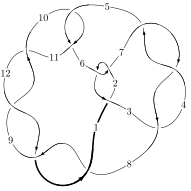
\includegraphics[width=112pt]{../../../GIT/diagram.site/Diagrams/png/1071_12a_0270.png}\\
\ \ \ A knot diagram\footnotemark}&
\allowdisplaybreaks
\textbf{Linearized knot diagam} \\
\cline{2-2}
 &
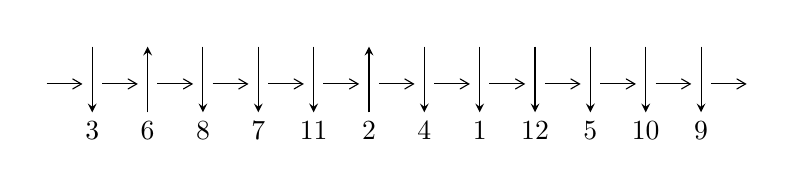
\begin{tikzpicture}[x=20pt, y=17pt]
	% nodes
	\node (C0) at (0, 0) {};
	\node (C1) at (1, 0) {};
	\node (C1U) at (1, +1) {};
	\node (C1D) at (1, -1) {3};

	\node (C2) at (2, 0) {};
	\node (C2U) at (2, +1) {};
	\node (C2D) at (2, -1) {6};

	\node (C3) at (3, 0) {};
	\node (C3U) at (3, +1) {};
	\node (C3D) at (3, -1) {8};

	\node (C4) at (4, 0) {};
	\node (C4U) at (4, +1) {};
	\node (C4D) at (4, -1) {7};

	\node (C5) at (5, 0) {};
	\node (C5U) at (5, +1) {};
	\node (C5D) at (5, -1) {11};

	\node (C6) at (6, 0) {};
	\node (C6U) at (6, +1) {};
	\node (C6D) at (6, -1) {2};

	\node (C7) at (7, 0) {};
	\node (C7U) at (7, +1) {};
	\node (C7D) at (7, -1) {4};

	\node (C8) at (8, 0) {};
	\node (C8U) at (8, +1) {};
	\node (C8D) at (8, -1) {1};

	\node (C9) at (9, 0) {};
	\node (C9U) at (9, +1) {};
	\node (C9D) at (9, -1) {12};

	\node (C10) at (10, 0) {};
	\node (C10U) at (10, +1) {};
	\node (C10D) at (10, -1) {5};

	\node (C11) at (11, 0) {};
	\node (C11U) at (11, +1) {};
	\node (C11D) at (11, -1) {10};

	\node (C12) at (12, 0) {};
	\node (C12U) at (12, +1) {};
	\node (C12D) at (12, -1) {9};
	\node (C13) at (13, 0) {};

	% arrows
	\draw[->,>={angle 60}]
	(C0) edge (C1) (C1) edge (C2) (C2) edge (C3) (C3) edge (C4) (C4) edge (C5) (C5) edge (C6) (C6) edge (C7) (C7) edge (C8) (C8) edge (C9) (C9) edge (C10) (C10) edge (C11) (C11) edge (C12) (C12) edge (C13) ;	\draw[->,>=stealth]
	(C1U) edge (C1D) (C2D) edge (C2U) (C3U) edge (C3D) (C4U) edge (C4D) (C5U) edge (C5D) (C6D) edge (C6U) (C7U) edge (C7D) (C8U) edge (C8D) (C9U) edge (C9D) (C10U) edge (C10D) (C11U) edge (C11D) (C12U) edge (C12D) ;
	\end{tikzpicture} \\
\hhline{~~} \\& 
\textbf{Solving Sequence} \\ \cline{2-2} 
 &
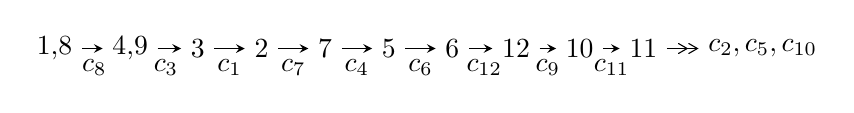
\begin{tikzpicture}[x=23pt, y=7pt]
	% node
	\node (A0) at (-1/8, 0) {1,8};
	\node (A1) at (17/16, 0) {4,9};
	\node (A2) at (17/8, 0) {3};
	\node (A3) at (25/8, 0) {2};
	\node (A4) at (33/8, 0) {7};
	\node (A5) at (41/8, 0) {5};
	\node (A6) at (49/8, 0) {6};
	\node (A7) at (57/8, 0) {12};
	\node (A8) at (65/8, 0) {10};
	\node (A9) at (73/8, 0) {11};
	\node (C1) at (1/2, -1) {$c_{8}$};
	\node (C2) at (13/8, -1) {$c_{3}$};
	\node (C3) at (21/8, -1) {$c_{1}$};
	\node (C4) at (29/8, -1) {$c_{7}$};
	\node (C5) at (37/8, -1) {$c_{4}$};
	\node (C6) at (45/8, -1) {$c_{6}$};
	\node (C7) at (53/8, -1) {$c_{12}$};
	\node (C8) at (61/8, -1) {$c_{9}$};
	\node (C9) at (69/8, -1) {$c_{11}$};
	\node (A10) at (11, 0) {$c_{2},c_{5},c_{10}$};

	% edge
	\draw[->,>=stealth]	
	(A0) edge (A1) (A1) edge (A2) (A2) edge (A3) (A3) edge (A4) (A4) edge (A5) (A5) edge (A6) (A6) edge (A7) (A7) edge (A8) (A8) edge (A9) ;
	\draw[->>,>={angle 60}]	
	(A9) edge (A10);
\end{tikzpicture} \\ 

\end{tabular} \\

\footnotetext{
The image of knot diagram is generated by the software ``\textbf{Draw programme}" developed by Andrew Bartholomew(\url{http://www.layer8.co.uk/maths/draw/index.htm\#Running-draw}), where we modified some parts for our purpose(\url{https://github.com/CATsTAILs/LinksPainter}).
}\phantom \\ \newline 
\centering \textbf{Ideals for irreducible components\footnotemark of $X_{\text{par}}$} 
 
\begin{align*}
I^u_{1}&=\langle 
-798268399 u^{41}+6250449929 u^{40}+\cdots+10357680512 b-2584646788,\\
\phantom{I^u_{1}}&\phantom{= \langle  }-358149411 u^{41}+2967411165 u^{40}+\cdots+5178840256 a-14354766596,\\
\phantom{I^u_{1}}&\phantom{= \langle  }u^{42}-8 u^{41}+\cdots+19 u+4\rangle \\
I^u_{2}&=\langle 
u^4 a^2-3 u^3 a^2+3 u^4 a+4 a^2 u^2+2 u^4-5 a^2 u+3 u^2 a-6 u^3+a^2+3 a u+8 u^2+3 b-3 a-10 u+2,\\
\phantom{I^u_{2}}&\phantom{= \langle  }2 u^4 a^2-2 u^3 a^2+3 u^4 a+8 a^2 u^2-2 u^3 a+a^3-6 a^2 u+11 u^2 a+6 a^2-5 a u+10 a+u,\\
\phantom{I^u_{2}}&\phantom{= \langle  }u^5- u^4+4 u^3-3 u^2+3 u-1\rangle \\
I^u_{3}&=\langle 
- u^3+u^2+b+a-3 u+2,\;-2 u^3 a+2 u^2 a-2 u^3+a^2-6 a u+u^2+4 a-5 u+2,\;u^4- u^3+3 u^2-2 u+1\rangle \\
\\
\end{align*}
\raggedright * 3 irreducible components of $\dim_{\mathbb{C}}=0$, with total 65 representations.\\
\footnotetext{All coefficients of polynomials are rational numbers. But the coefficients are sometimes approximated in decimal forms when there is not enough margin.}
\newpage
\renewcommand{\arraystretch}{1}
\centering \section*{I. $I^u_{1}= \langle -7.98\times10^{8} u^{41}+6.25\times10^{9} u^{40}+\cdots+1.04\times10^{10} b-2.58\times10^{9},\;-3.58\times10^{8} u^{41}+2.97\times10^{9} u^{40}+\cdots+5.18\times10^{9} a-1.44\times10^{10},\;u^{42}-8 u^{41}+\cdots+19 u+4 \rangle$}
\flushleft \textbf{(i) Arc colorings}\\
\begin{tabular}{m{7pt} m{180pt} m{7pt} m{180pt} }
\flushright $a_{1}=$&$\begin{pmatrix}0\\u\end{pmatrix}$ \\
\flushright $a_{8}=$&$\begin{pmatrix}1\\0\end{pmatrix}$ \\
\flushright $a_{4}=$&$\begin{pmatrix}0.0691563 u^{41}-0.572988 u^{40}+\cdots+3.90826 u+2.77181\\0.0770702 u^{41}-0.603460 u^{40}+\cdots-0.703314 u+0.249539\end{pmatrix}$ \\
\flushright $a_{9}=$&$\begin{pmatrix}1\\u^2\end{pmatrix}$ \\
\flushright $a_{3}=$&$\begin{pmatrix}0.146226 u^{41}-1.17645 u^{40}+\cdots+3.20495 u+3.02135\\0.0770702 u^{41}-0.603460 u^{40}+\cdots-0.703314 u+0.249539\end{pmatrix}$ \\
\flushright $a_{2}=$&$\begin{pmatrix}0.0816169 u^{41}-0.664619 u^{40}+\cdots+6.14207 u+0.645428\\0.0288129 u^{41}-0.231921 u^{40}+\cdots+1.24875 u+0.105032\end{pmatrix}$ \\
\flushright $a_{7}=$&$\begin{pmatrix}-0.0196220 u^{41}+0.147935 u^{40}+\cdots-6.11036 u+0.584750\\-0.00663609 u^{41}+0.0909429 u^{40}+\cdots+1.05555 u+0.165094\end{pmatrix}$ \\
\flushright $a_{5}=$&$\begin{pmatrix}0.0115304 u^{41}-0.109146 u^{40}+\cdots+7.16076 u+1.81175\\0.0576259 u^{41}-0.463842 u^{40}+\cdots-0.502505 u+0.210065\end{pmatrix}$ \\
\flushright $a_{6}=$&$\begin{pmatrix}-0.0525162 u^{41}+0.477755 u^{40}+\cdots-5.10962 u-1.50031\\-0.0197372 u^{41}+0.196786 u^{40}+\cdots+0.707841 u-0.276625\end{pmatrix}$ \\
\flushright $a_{12}=$&$\begin{pmatrix}u\\u^3+u\end{pmatrix}$ \\
\flushright $a_{10}=$&$\begin{pmatrix}u^2+1\\u^4+2 u^2\end{pmatrix}$ \\
\flushright $a_{11}=$&$\begin{pmatrix}u^3+2 u\\u^5+3 u^3+u\end{pmatrix}$\\&\end{tabular}
\flushleft \textbf{(ii) Obstruction class $= -1$}\\~\\
\flushleft \textbf{(iii) Cusp Shapes $= \frac{1891553825}{2589420128} u^{41}-\frac{14308919975}{2589420128} u^{40}+\cdots+\frac{33847466689}{2589420128} u-\frac{1329586633}{647355032}$}\\~\\
\newpage\renewcommand{\arraystretch}{1}
\flushleft \textbf{(iv) u-Polynomials at the component}\newline \\
\begin{tabular}{m{50pt}|m{274pt}}
Crossings & \hspace{64pt}u-Polynomials at each crossing \\
\hline $$\begin{aligned}c_{1}\end{aligned}$$&$\begin{aligned}
&u^{42}+13 u^{41}+\cdots+147 u+4
\end{aligned}$\\
\hline $$\begin{aligned}c_{2},c_{6}\end{aligned}$$&$\begin{aligned}
&u^{42}- u^{41}+\cdots-11 u+2
\end{aligned}$\\
\hline $$\begin{aligned}c_{3},c_{4},c_{7}\end{aligned}$$&$\begin{aligned}
&u^{42}- u^{41}+\cdots-17 u+2
\end{aligned}$\\
\hline $$\begin{aligned}c_{5},c_{10}\end{aligned}$$&$\begin{aligned}
&u^{42}-2 u^{41}+\cdots- u+2
\end{aligned}$\\
\hline $$\begin{aligned}c_{8},c_{9},c_{11}\\c_{12}\end{aligned}$$&$\begin{aligned}
&u^{42}+8 u^{41}+\cdots-19 u+4
\end{aligned}$\\
\hline
\end{tabular}\\~\\
\newpage\renewcommand{\arraystretch}{1}
\flushleft \textbf{(v) Riley Polynomials at the component}\newline \\
\begin{tabular}{m{50pt}|m{274pt}}
Crossings & \hspace{64pt}Riley Polynomials at each crossing \\
\hline $$\begin{aligned}c_{1}\end{aligned}$$&$\begin{aligned}
&y^{42}+41 y^{41}+\cdots-1601 y+16
\end{aligned}$\\
\hline $$\begin{aligned}c_{2},c_{6}\end{aligned}$$&$\begin{aligned}
&y^{42}+13 y^{41}+\cdots+147 y+4
\end{aligned}$\\
\hline $$\begin{aligned}c_{3},c_{4},c_{7}\end{aligned}$$&$\begin{aligned}
&y^{42}+49 y^{41}+\cdots+163 y+4
\end{aligned}$\\
\hline $$\begin{aligned}c_{5},c_{10}\end{aligned}$$&$\begin{aligned}
&y^{42}-8 y^{41}+\cdots+19 y+4
\end{aligned}$\\
\hline $$\begin{aligned}c_{8},c_{9},c_{11}\\c_{12}\end{aligned}$$&$\begin{aligned}
&y^{42}+52 y^{41}+\cdots-593 y+16
\end{aligned}$\\
\hline
\end{tabular}\\~\\
\newpage\flushleft \textbf{(vi) Complex Volumes and Cusp Shapes}
$$\begin{array}{c|c|c}  
\text{Solutions to }I^u_{1}& \I (\text{vol} + \sqrt{-1}CS) & \text{Cusp shape}\\
 \hline 
\begin{aligned}
u &= -0.199296 + 0.987147 I \\
a &= -1.16462 - 1.63691 I \\
b &= -0.07090 + 1.52196 I\end{aligned}
 & \phantom{-}9.23309 - 0.66880 I & \phantom{-0.000000 -}0. + 2.09820 I \\ \hline\begin{aligned}
u &= -0.199296 - 0.987147 I \\
a &= -1.16462 + 1.63691 I \\
b &= -0.07090 - 1.52196 I\end{aligned}
 & \phantom{-}9.23309 + 0.66880 I & \phantom{-0.000000 } 0. - 2.09820 I \\ \hline\begin{aligned}
u &= \phantom{-}0.838964 + 0.514549 I \\
a &= \phantom{-}0.469470 - 0.436996 I \\
b &= -0.043564 + 1.403040 I\end{aligned}
 & \phantom{-}2.90089 - 0.20752 I & -6.26688 + 0. I\phantom{ +0.000000I} \\ \hline\begin{aligned}
u &= \phantom{-}0.838964 - 0.514549 I \\
a &= \phantom{-}0.469470 + 0.436996 I \\
b &= -0.043564 - 1.403040 I\end{aligned}
 & \phantom{-}2.90089 + 0.20752 I & -6.26688 + 0. I\phantom{ +0.000000I} \\ \hline\begin{aligned}
u &= \phantom{-}0.915478 + 0.320876 I \\
a &= -0.717082 + 0.350239 I \\
b &= -0.16817 - 1.42645 I\end{aligned}
 & \phantom{-}2.31734 - 5.40050 I & -8.00000 + 6.13743 I \\ \hline\begin{aligned}
u &= \phantom{-}0.915478 - 0.320876 I \\
a &= -0.717082 - 0.350239 I \\
b &= -0.16817 + 1.42645 I\end{aligned}
 & \phantom{-}2.31734 + 5.40050 I & -8.00000 - 6.13743 I \\ \hline\begin{aligned}
u &= \phantom{-}0.450384 + 1.002590 I \\
a &= -0.392271 + 0.489442 I \\
b &= -0.762687 - 0.383581 I\end{aligned}
 & \phantom{-}0.60208 - 6.73872 I & \phantom{-0.000000 } 0 \\ \hline\begin{aligned}
u &= \phantom{-}0.450384 - 1.002590 I \\
a &= -0.392271 - 0.489442 I \\
b &= -0.762687 + 0.383581 I\end{aligned}
 & \phantom{-}0.60208 + 6.73872 I & \phantom{-0.000000 } 0 \\ \hline\begin{aligned}
u &= -0.302006 + 0.836923 I \\
a &= \phantom{-}1.67864 + 1.44506 I \\
b &= \phantom{-}0.22550 - 1.51897 I\end{aligned}
 & \phantom{-}8.07529 + 5.48503 I & -0.70916 - 2.91852 I \\ \hline\begin{aligned}
u &= -0.302006 - 0.836923 I \\
a &= \phantom{-}1.67864 - 1.44506 I \\
b &= \phantom{-}0.22550 + 1.51897 I\end{aligned}
 & \phantom{-}8.07529 - 5.48503 I & -0.70916 + 2.91852 I\\
 \hline 
 \end{array}$$\newpage$$\begin{array}{c|c|c}  
\text{Solutions to }I^u_{1}& \I (\text{vol} + \sqrt{-1}CS) & \text{Cusp shape}\\
 \hline 
\begin{aligned}
u &= -0.060244 + 0.788682 I \\
a &= \phantom{-}0.605228 + 0.925856 I \\
b &= \phantom{-}0.693973 - 0.485377 I\end{aligned}
 & \phantom{-}1.48615 + 2.15029 I & -3.71859 - 3.19032 I \\ \hline\begin{aligned}
u &= -0.060244 - 0.788682 I \\
a &= \phantom{-}0.605228 - 0.925856 I \\
b &= \phantom{-}0.693973 + 0.485377 I\end{aligned}
 & \phantom{-}1.48615 - 2.15029 I & -3.71859 + 3.19032 I \\ \hline\begin{aligned}
u &= \phantom{-}0.509270 + 0.583804 I \\
a &= -0.220296 + 1.029270 I \\
b &= -0.264495 + 0.109372 I\end{aligned}
 & -1.98852 - 1.21898 I & -14.0512 + 3.6292 I \\ \hline\begin{aligned}
u &= \phantom{-}0.509270 - 0.583804 I \\
a &= -0.220296 - 1.029270 I \\
b &= -0.264495 - 0.109372 I\end{aligned}
 & -1.98852 + 1.21898 I & -14.0512 - 3.6292 I \\ \hline\begin{aligned}
u &= \phantom{-}0.588709 + 1.120860 I \\
a &= -1.07852 + 1.38460 I \\
b &= -0.26708 - 1.48568 I\end{aligned}
 & \phantom{-}6.68238 - 10.46650 I & \phantom{-0.000000 } 0 \\ \hline\begin{aligned}
u &= \phantom{-}0.588709 - 1.120860 I \\
a &= -1.07852 - 1.38460 I \\
b &= -0.26708 + 1.48568 I\end{aligned}
 & \phantom{-}6.68238 + 10.46650 I & \phantom{-0.000000 } 0 \\ \hline\begin{aligned}
u &= \phantom{-}0.701442 + 0.208159 I \\
a &= -0.779517 - 0.388802 I \\
b &= -0.556875 - 0.244623 I\end{aligned}
 & -3.10427 - 2.84153 I & -15.5735 + 6.4385 I \\ \hline\begin{aligned}
u &= \phantom{-}0.701442 - 0.208159 I \\
a &= -0.779517 + 0.388802 I \\
b &= -0.556875 + 0.244623 I\end{aligned}
 & -3.10427 + 2.84153 I & -15.5735 - 6.4385 I \\ \hline\begin{aligned}
u &= \phantom{-}0.439199 + 1.197000 I \\
a &= \phantom{-}0.69981 - 1.54440 I \\
b &= \phantom{-}0.13274 + 1.47292 I\end{aligned}
 & \phantom{-}8.27660 - 4.56148 I & \phantom{-0.000000 } 0 \\ \hline\begin{aligned}
u &= \phantom{-}0.439199 - 1.197000 I \\
a &= \phantom{-}0.69981 + 1.54440 I \\
b &= \phantom{-}0.13274 - 1.47292 I\end{aligned}
 & \phantom{-}8.27660 + 4.56148 I & \phantom{-0.000000 } 0\\
 \hline 
 \end{array}$$\newpage$$\begin{array}{c|c|c}  
\text{Solutions to }I^u_{1}& \I (\text{vol} + \sqrt{-1}CS) & \text{Cusp shape}\\
 \hline 
\begin{aligned}
u &= \phantom{-}0.220775 + 0.575673 I \\
a &= -0.342696 - 0.818451 I \\
b &= \phantom{-}0.139249 + 0.831769 I\end{aligned}
 & \phantom{-}1.40137 - 1.70947 I & -0.06449 + 5.59686 I \\ \hline\begin{aligned}
u &= \phantom{-}0.220775 - 0.575673 I \\
a &= -0.342696 + 0.818451 I \\
b &= \phantom{-}0.139249 - 0.831769 I\end{aligned}
 & \phantom{-}1.40137 + 1.70947 I & -0.06449 - 5.59686 I \\ \hline\begin{aligned}
u &= \phantom{-}0.11412 + 1.52011 I \\
a &= \phantom{-}0.001825 - 1.058650 I \\
b &= \phantom{-}0.013978 + 1.115610 I\end{aligned}
 & \phantom{-}8.31413 - 3.12469 I & \phantom{-0.000000 } 0 \\ \hline\begin{aligned}
u &= \phantom{-}0.11412 - 1.52011 I \\
a &= \phantom{-}0.001825 + 1.058650 I \\
b &= \phantom{-}0.013978 - 1.115610 I\end{aligned}
 & \phantom{-}8.31413 + 3.12469 I & \phantom{-0.000000 } 0 \\ \hline\begin{aligned}
u &= -0.453394 + 0.093145 I \\
a &= -0.29248 + 1.41477 I \\
b &= \phantom{-}0.09646 + 1.48180 I\end{aligned}
 & \phantom{-}5.82303 - 2.87870 I & \phantom{-}0.05391 + 2.88471 I \\ \hline\begin{aligned}
u &= -0.453394 - 0.093145 I \\
a &= -0.29248 - 1.41477 I \\
b &= \phantom{-}0.09646 - 1.48180 I\end{aligned}
 & \phantom{-}5.82303 + 2.87870 I & \phantom{-}0.05391 - 2.88471 I \\ \hline\begin{aligned}
u &= \phantom{-}0.09947 + 1.57211 I \\
a &= -0.005582 + 0.932064 I \\
b &= -0.027777 - 0.190004 I\end{aligned}
 & \phantom{-}5.22550 - 3.18763 I & \phantom{-0.000000 } 0 \\ \hline\begin{aligned}
u &= \phantom{-}0.09947 - 1.57211 I \\
a &= -0.005582 - 0.932064 I \\
b &= -0.027777 + 0.190004 I\end{aligned}
 & \phantom{-}5.22550 + 3.18763 I & \phantom{-0.000000 } 0 \\ \hline\begin{aligned}
u &= -0.01154 + 1.67140 I \\
a &= -0.049530 + 0.747153 I \\
b &= \phantom{-}0.911882 - 0.498339 I\end{aligned}
 & \phantom{-}10.24920 + 2.39200 I & \phantom{-0.000000 } 0 \\ \hline\begin{aligned}
u &= -0.01154 - 1.67140 I \\
a &= -0.049530 - 0.747153 I \\
b &= \phantom{-}0.911882 + 0.498339 I\end{aligned}
 & \phantom{-}10.24920 - 2.39200 I & \phantom{-0.000000 } 0\\
 \hline 
 \end{array}$$\newpage$$\begin{array}{c|c|c}  
\text{Solutions to }I^u_{1}& \I (\text{vol} + \sqrt{-1}CS) & \text{Cusp shape}\\
 \hline 
\begin{aligned}
u &= -0.08120 + 1.67874 I \\
a &= \phantom{-}0.80016 + 1.97320 I \\
b &= \phantom{-}0.33059 - 1.55890 I\end{aligned}
 & \phantom{-}16.9456 + 6.9601 I & \phantom{-0.000000 } 0 \\ \hline\begin{aligned}
u &= -0.08120 - 1.67874 I \\
a &= \phantom{-}0.80016 - 1.97320 I \\
b &= \phantom{-}0.33059 + 1.55890 I\end{aligned}
 & \phantom{-}16.9456 - 6.9601 I & \phantom{-0.000000 } 0 \\ \hline\begin{aligned}
u &= \phantom{-}0.12364 + 1.71287 I \\
a &= \phantom{-}0.056715 + 0.692130 I \\
b &= -0.920998 - 0.474791 I\end{aligned}
 & \phantom{-}10.09190 - 9.06080 I & \phantom{-0.000000 } 0 \\ \hline\begin{aligned}
u &= \phantom{-}0.12364 - 1.71287 I \\
a &= \phantom{-}0.056715 - 0.692130 I \\
b &= -0.920998 + 0.474791 I\end{aligned}
 & \phantom{-}10.09190 + 9.06080 I & \phantom{-0.000000 } 0 \\ \hline\begin{aligned}
u &= -0.03891 + 1.71786 I \\
a &= -0.51740 - 2.10632 I \\
b &= -0.20263 + 1.61169 I\end{aligned}
 & \phantom{-}18.9080 + 0.2132 I & \phantom{-0.000000 } 0 \\ \hline\begin{aligned}
u &= -0.03891 - 1.71786 I \\
a &= -0.51740 + 2.10632 I \\
b &= -0.20263 - 1.61169 I\end{aligned}
 & \phantom{-}18.9080 - 0.2132 I & \phantom{-0.000000 } 0 \\ \hline\begin{aligned}
u &= \phantom{-}0.17216 + 1.75098 I \\
a &= -0.74841 + 1.91623 I \\
b &= -0.34100 - 1.54865 I\end{aligned}
 & \phantom{-}16.6556 - 13.6886 I & \phantom{-0.000000 } 0 \\ \hline\begin{aligned}
u &= \phantom{-}0.17216 - 1.75098 I \\
a &= -0.74841 - 1.91623 I \\
b &= -0.34100 + 1.54865 I\end{aligned}
 & \phantom{-}16.6556 + 13.6886 I & \phantom{-0.000000 } 0 \\ \hline\begin{aligned}
u &= \phantom{-}0.12140 + 1.76169 I \\
a &= \phantom{-}0.47312 - 2.07005 I \\
b &= \phantom{-}0.21928 + 1.60308 I\end{aligned}
 & \phantom{-}18.7265 - 6.9926 I & \phantom{-0.000000 } 0 \\ \hline\begin{aligned}
u &= \phantom{-}0.12140 - 1.76169 I \\
a &= \phantom{-}0.47312 + 2.07005 I \\
b &= \phantom{-}0.21928 - 1.60308 I\end{aligned}
 & \phantom{-}18.7265 + 6.9926 I & \phantom{-0.000000 } 0\\
 \hline 
 \end{array}$$\newpage$$\begin{array}{c|c|c}  
\text{Solutions to }I^u_{1}& \I (\text{vol} + \sqrt{-1}CS) & \text{Cusp shape}\\
 \hline 
\begin{aligned}
u &= -0.148412 + 0.075498 I \\
a &= \phantom{-}1.14844 + 3.46411 I \\
b &= \phantom{-}0.362523 + 0.421697 I\end{aligned}
 & -0.422743 - 1.307230 I & -4.54925 + 5.05506 I \\ \hline\begin{aligned}
u &= -0.148412 - 0.075498 I \\
a &= \phantom{-}1.14844 - 3.46411 I \\
b &= \phantom{-}0.362523 - 0.421697 I\end{aligned}
 & -0.422743 + 1.307230 I & -4.54925 - 5.05506 I\\
 \hline 
 \end{array}$$\newpage\newpage\renewcommand{\arraystretch}{1}
\centering \section*{II. $I^u_{2}= \langle u^4 a^2+3 u^4 a+\cdots-3 a+2,\;2 u^4 a^2+3 u^4 a+\cdots+6 a^2+10 a,\;u^5- u^4+4 u^3-3 u^2+3 u-1 \rangle$}
\flushleft \textbf{(i) Arc colorings}\\
\begin{tabular}{m{7pt} m{180pt} m{7pt} m{180pt} }
\flushright $a_{1}=$&$\begin{pmatrix}0\\u\end{pmatrix}$ \\
\flushright $a_{8}=$&$\begin{pmatrix}1\\0\end{pmatrix}$ \\
\flushright $a_{4}=$&$\begin{pmatrix}a\\-\frac{1}{3} u^4 a^2- u^4 a+\cdots+a-\frac{2}{3}\end{pmatrix}$ \\
\flushright $a_{9}=$&$\begin{pmatrix}1\\u^2\end{pmatrix}$ \\
\flushright $a_{3}=$&$\begin{pmatrix}-\frac{1}{3} u^4 a^2- u^4 a+\cdots+2 a-\frac{2}{3}\\-\frac{1}{3} u^4 a^2- u^4 a+\cdots+a-\frac{2}{3}\end{pmatrix}$ \\
\flushright $a_{2}=$&$\begin{pmatrix}a\\-\frac{1}{3} u^4 a^2- u^4 a+\cdots+a-\frac{2}{3}\end{pmatrix}$ \\
\flushright $a_{7}=$&$\begin{pmatrix}\frac{1}{3} u^4 a^2+\frac{2}{3} u^4+\cdots+a+\frac{2}{3}\\-\frac{2}{3} u^4 a^2+u^4 a+\cdots+a+\frac{2}{3}\end{pmatrix}$ \\
\flushright $a_{5}=$&$\begin{pmatrix}- u\\u\end{pmatrix}$ \\
\flushright $a_{6}=$&$\begin{pmatrix}1\\0\end{pmatrix}$ \\
\flushright $a_{12}=$&$\begin{pmatrix}u\\u^3+u\end{pmatrix}$ \\
\flushright $a_{10}=$&$\begin{pmatrix}u^2+1\\u^4+2 u^2\end{pmatrix}$ \\
\flushright $a_{11}=$&$\begin{pmatrix}u^3+2 u\\u^4- u^3+3 u^2-2 u+1\end{pmatrix}$\\&\end{tabular}
\flushleft \textbf{(ii) Obstruction class $= -1$}\\~\\
\flushleft \textbf{(iii) Cusp Shapes $= -4 u^4+4 u^3-16 u^2+12 u-14$}\\~\\
\newpage\renewcommand{\arraystretch}{1}
\flushleft \textbf{(iv) u-Polynomials at the component}\newline \\
\begin{tabular}{m{50pt}|m{274pt}}
Crossings & \hspace{64pt}u-Polynomials at each crossing \\
\hline $$\begin{aligned}c_{1}\end{aligned}$$&$\begin{aligned}
&u^{15}+10 u^{14}+\cdots+3 u-1
\end{aligned}$\\
\hline $$\begin{aligned}c_{2},c_{3},c_{4}\\c_{6},c_{7}\end{aligned}$$&$\begin{aligned}
&u^{15}+5 u^{13}+\cdots+3 u+1
\end{aligned}$\\
\hline $$\begin{aligned}c_{5},c_{10}\end{aligned}$$&$\begin{aligned}
&(u^5+u^4- u^2+u+1)^3
\end{aligned}$\\
\hline $$\begin{aligned}c_{8},c_{9},c_{11}\\c_{12}\end{aligned}$$&$\begin{aligned}
&(u^5+u^4+4 u^3+3 u^2+3 u+1)^3
\end{aligned}$\\
\hline
\end{tabular}\\~\\
\newpage\renewcommand{\arraystretch}{1}
\flushleft \textbf{(v) Riley Polynomials at the component}\newline \\
\begin{tabular}{m{50pt}|m{274pt}}
Crossings & \hspace{64pt}Riley Polynomials at each crossing \\
\hline $$\begin{aligned}c_{1}\end{aligned}$$&$\begin{aligned}
&y^{15}-10 y^{14}+\cdots+47 y-1
\end{aligned}$\\
\hline $$\begin{aligned}c_{2},c_{3},c_{4}\\c_{6},c_{7}\end{aligned}$$&$\begin{aligned}
&y^{15}+10 y^{14}+\cdots+3 y-1
\end{aligned}$\\
\hline $$\begin{aligned}c_{5},c_{10}\end{aligned}$$&$\begin{aligned}
&(y^5- y^4+4 y^3-3 y^2+3 y-1)^3
\end{aligned}$\\
\hline $$\begin{aligned}c_{8},c_{9},c_{11}\\c_{12}\end{aligned}$$&$\begin{aligned}
&(y^5+7 y^4+16 y^3+13 y^2+3 y-1)^3
\end{aligned}$\\
\hline
\end{tabular}\\~\\
\newpage\flushleft \textbf{(vi) Complex Volumes and Cusp Shapes}
$$\begin{array}{c|c|c}  
\text{Solutions to }I^u_{2}& \I (\text{vol} + \sqrt{-1}CS) & \text{Cusp shape}\\
 \hline 
\begin{aligned}
u &= \phantom{-}0.233677 + 0.885557 I \\
a &= -0.387789 - 0.623465 I \\
b &= -0.497623 + 0.756574 I\end{aligned}
 & \phantom{-}1.81981 - 2.21397 I & -3.11432 + 4.22289 I \\ \hline\begin{aligned}
u &= \phantom{-}0.233677 + 0.885557 I \\
a &= \phantom{-}0.085680 - 0.388688 I \\
b &= \phantom{-}0.555046 + 0.543774 I\end{aligned}
 & \phantom{-}1.81981 - 2.21397 I & -3.11432 + 4.22289 I \\ \hline\begin{aligned}
u &= \phantom{-}0.233677 + 0.885557 I \\
a &= -0.25505 + 3.12360 I \\
b &= -0.057423 - 1.300350 I\end{aligned}
 & \phantom{-}1.81981 - 2.21397 I & -3.11432 + 4.22289 I \\ \hline\begin{aligned}
u &= \phantom{-}0.233677 - 0.885557 I \\
a &= -0.387789 + 0.623465 I \\
b &= -0.497623 - 0.756574 I\end{aligned}
 & \phantom{-}1.81981 + 2.21397 I & -3.11432 - 4.22289 I \\ \hline\begin{aligned}
u &= \phantom{-}0.233677 - 0.885557 I \\
a &= \phantom{-}0.085680 + 0.388688 I \\
b &= \phantom{-}0.555046 - 0.543774 I\end{aligned}
 & \phantom{-}1.81981 + 2.21397 I & -3.11432 - 4.22289 I \\ \hline\begin{aligned}
u &= \phantom{-}0.233677 - 0.885557 I \\
a &= -0.25505 - 3.12360 I \\
b &= -0.057423 + 1.300350 I\end{aligned}
 & \phantom{-}1.81981 + 2.21397 I & -3.11432 - 4.22289 I \\ \hline\begin{aligned}
u &= \phantom{-}0.416284\phantom{ +0.000000I} \\
a &= -0.0435290\phantom{ +0.000000I} \\
b &= \phantom{-}0.366895\phantom{ +0.000000I}\end{aligned}
 & -0.882183\phantom{ +0.000000I} & -11.6090\phantom{ +0.000000I} \\ \hline\begin{aligned}
u &= \phantom{-}0.416284\phantom{ +0.000000I} \\
a &= -2.38044 + 1.97405 I \\
b &= -0.183448 - 1.049270 I\end{aligned}
 & -0.882183\phantom{ +0.000000I} & -11.6090\phantom{ +0.000000I} \\ \hline\begin{aligned}
u &= \phantom{-}0.416284\phantom{ +0.000000I} \\
a &= -2.38044 - 1.97405 I \\
b &= -0.183448 + 1.049270 I\end{aligned}
 & -0.882183\phantom{ +0.000000I} & -11.6090\phantom{ +0.000000I} \\ \hline\begin{aligned}
u &= \phantom{-}0.05818 + 1.69128 I \\
a &= \phantom{-}0.091113 - 0.799543 I \\
b &= -0.778812 + 0.748610 I\end{aligned}
 & \phantom{-}10.95830 - 3.33174 I & -2.08126 + 2.36228 I\\
 \hline 
 \end{array}$$\newpage$$\begin{array}{c|c|c}  
\text{Solutions to }I^u_{2}& \I (\text{vol} + \sqrt{-1}CS) & \text{Cusp shape}\\
 \hline 
\begin{aligned}
u &= \phantom{-}0.05818 + 1.69128 I \\
a &= -0.117137 - 0.758678 I \\
b &= \phantom{-}0.789470 + 0.718695 I\end{aligned}
 & \phantom{-}10.95830 - 3.33174 I & -2.08126 + 2.36228 I \\ \hline\begin{aligned}
u &= \phantom{-}0.05818 + 1.69128 I \\
a &= -0.01461 + 2.73936 I \\
b &= -0.01066 - 1.46731 I\end{aligned}
 & \phantom{-}10.95830 - 3.33174 I & -2.08126 + 2.36228 I \\ \hline\begin{aligned}
u &= \phantom{-}0.05818 - 1.69128 I \\
a &= \phantom{-}0.091113 + 0.799543 I \\
b &= -0.778812 - 0.748610 I\end{aligned}
 & \phantom{-}10.95830 + 3.33174 I & -2.08126 - 2.36228 I \\ \hline\begin{aligned}
u &= \phantom{-}0.05818 - 1.69128 I \\
a &= -0.117137 + 0.758678 I \\
b &= \phantom{-}0.789470 - 0.718695 I\end{aligned}
 & \phantom{-}10.95830 + 3.33174 I & -2.08126 - 2.36228 I \\ \hline\begin{aligned}
u &= \phantom{-}0.05818 - 1.69128 I \\
a &= -0.01461 - 2.73936 I \\
b &= -0.01066 + 1.46731 I\end{aligned}
 & \phantom{-}10.95830 + 3.33174 I & -2.08126 - 2.36228 I\\
 \hline 
 \end{array}$$\newpage\newpage\renewcommand{\arraystretch}{1}
\centering \section*{III. $I^u_{3}= \langle - u^3+u^2+b+a-3 u+2,\;-2 u^3 a-2 u^3+\cdots+4 a+2,\;u^4- u^3+3 u^2-2 u+1 \rangle$}
\flushleft \textbf{(i) Arc colorings}\\
\begin{tabular}{m{7pt} m{180pt} m{7pt} m{180pt} }
\flushright $a_{1}=$&$\begin{pmatrix}0\\u\end{pmatrix}$ \\
\flushright $a_{8}=$&$\begin{pmatrix}1\\0\end{pmatrix}$ \\
\flushright $a_{4}=$&$\begin{pmatrix}a\\u^3- u^2- a+3 u-2\end{pmatrix}$ \\
\flushright $a_{9}=$&$\begin{pmatrix}1\\u^2\end{pmatrix}$ \\
\flushright $a_{3}=$&$\begin{pmatrix}u^3- u^2+3 u-2\\u^3- u^2- a+3 u-2\end{pmatrix}$ \\
\flushright $a_{2}=$&$\begin{pmatrix}u^3- u^2+3 u-2\\u^3- u^2- a+4 u-2\end{pmatrix}$ \\
\flushright $a_{7}=$&$\begin{pmatrix}u^3 a- u^2 a+2 u^3+3 a u- u^2-2 a+5 u-1\\1\end{pmatrix}$ \\
\flushright $a_{5}=$&$\begin{pmatrix}- u^3+u^2+a-3 u+2\\0\end{pmatrix}$ \\
\flushright $a_{6}=$&$\begin{pmatrix}0\\- a u-1\end{pmatrix}$ \\
\flushright $a_{12}=$&$\begin{pmatrix}u\\u^3+u\end{pmatrix}$ \\
\flushright $a_{10}=$&$\begin{pmatrix}u^2+1\\u^3- u^2+2 u-1\end{pmatrix}$ \\
\flushright $a_{11}=$&$\begin{pmatrix}u^3+2 u\\u^3- u^2+2 u-1\end{pmatrix}$\\&\end{tabular}
\flushleft \textbf{(ii) Obstruction class $= 1$}\\~\\
\flushleft \textbf{(iii) Cusp Shapes $= 4 u^3-4 u^2+12 u-12$}\\~\\
\newpage\renewcommand{\arraystretch}{1}
\flushleft \textbf{(iv) u-Polynomials at the component}\newline \\
\begin{tabular}{m{50pt}|m{274pt}}
Crossings & \hspace{64pt}u-Polynomials at each crossing \\
\hline $$\begin{aligned}c_{1}\end{aligned}$$&$\begin{aligned}
&(u-1)^8
\end{aligned}$\\
\hline $$\begin{aligned}c_{2},c_{3},c_{4}\\c_{6},c_{7}\end{aligned}$$&$\begin{aligned}
&(u^2+1)^4
\end{aligned}$\\
\hline $$\begin{aligned}c_{5},c_{10}\end{aligned}$$&$\begin{aligned}
&u^8- u^6+3 u^4-2 u^2+1
\end{aligned}$\\
\hline $$\begin{aligned}c_{8},c_{9}\end{aligned}$$&$\begin{aligned}
&(u^4- u^3+3 u^2-2 u+1)^2
\end{aligned}$\\
\hline $$\begin{aligned}c_{11},c_{12}\end{aligned}$$&$\begin{aligned}
&(u^4+u^3+3 u^2+2 u+1)^2
\end{aligned}$\\
\hline
\end{tabular}\\~\\
\newpage\renewcommand{\arraystretch}{1}
\flushleft \textbf{(v) Riley Polynomials at the component}\newline \\
\begin{tabular}{m{50pt}|m{274pt}}
Crossings & \hspace{64pt}Riley Polynomials at each crossing \\
\hline $$\begin{aligned}c_{1}\end{aligned}$$&$\begin{aligned}
&(y-1)^8
\end{aligned}$\\
\hline $$\begin{aligned}c_{2},c_{3},c_{4}\\c_{6},c_{7}\end{aligned}$$&$\begin{aligned}
&(y+1)^8
\end{aligned}$\\
\hline $$\begin{aligned}c_{5},c_{10}\end{aligned}$$&$\begin{aligned}
&(y^4- y^3+3 y^2-2 y+1)^2
\end{aligned}$\\
\hline $$\begin{aligned}c_{8},c_{9},c_{11}\\c_{12}\end{aligned}$$&$\begin{aligned}
&(y^4+5 y^3+7 y^2+2 y+1)^2
\end{aligned}$\\
\hline
\end{tabular}\\~\\
\newpage\flushleft \textbf{(vi) Complex Volumes and Cusp Shapes}
$$\begin{array}{c|c|c}  
\text{Solutions to }I^u_{3}& \I (\text{vol} + \sqrt{-1}CS) & \text{Cusp shape}\\
 \hline 
\begin{aligned}
u &= \phantom{-}0.395123 + 0.506844 I \\
a &= -0.956685 + 0.227186 I \\
b &= \phantom{-0.000000 -}1.000000 I\end{aligned}
 & -0.21101 - 1.41510 I & -7.82674 + 4.90874 I \\ \hline\begin{aligned}
u &= \phantom{-}0.395123 + 0.506844 I \\
a &= -0.95668 + 2.22719 I \\
b &= \phantom{-0.000000 } -1.000000 I\end{aligned}
 & -0.21101 - 1.41510 I & -7.82674 + 4.90874 I \\ \hline\begin{aligned}
u &= \phantom{-}0.395123 - 0.506844 I \\
a &= -0.956685 - 0.227186 I \\
b &= \phantom{-0.000000 } -1.000000 I\end{aligned}
 & -0.21101 + 1.41510 I & -7.82674 - 4.90874 I \\ \hline\begin{aligned}
u &= \phantom{-}0.395123 - 0.506844 I \\
a &= -0.95668 - 2.22719 I \\
b &= \phantom{-0.000000 -}1.000000 I\end{aligned}
 & -0.21101 + 1.41510 I & -7.82674 - 4.90874 I \\ \hline\begin{aligned}
u &= \phantom{-}0.10488 + 1.55249 I \\
a &= -0.043315 - 0.358800 I \\
b &= \phantom{-0.000000 -}1.000000 I\end{aligned}
 & \phantom{-}6.79074 - 3.16396 I & -4.17326 + 2.56480 I \\ \hline\begin{aligned}
u &= \phantom{-}0.10488 + 1.55249 I \\
a &= -0.04332 + 1.64120 I \\
b &= \phantom{-0.000000 } -1.000000 I\end{aligned}
 & \phantom{-}6.79074 - 3.16396 I & -4.17326 + 2.56480 I \\ \hline\begin{aligned}
u &= \phantom{-}0.10488 - 1.55249 I \\
a &= -0.043315 + 0.358800 I \\
b &= \phantom{-0.000000 } -1.000000 I\end{aligned}
 & \phantom{-}6.79074 + 3.16396 I & -4.17326 - 2.56480 I \\ \hline\begin{aligned}
u &= \phantom{-}0.10488 - 1.55249 I \\
a &= -0.04332 - 1.64120 I \\
b &= \phantom{-0.000000 -}1.000000 I\end{aligned}
 & \phantom{-}6.79074 + 3.16396 I & -4.17326 - 2.56480 I\\
 \hline 
 \end{array}$$\newpage
\newpage\renewcommand{\arraystretch}{1}
\centering \section*{ IV. u-Polynomials}
\begin{tabular}{m{50pt}|m{274pt}}
Crossings & \hspace{64pt}u-Polynomials at each crossing \\
\hline $$\begin{aligned}c_{1}\end{aligned}$$&$\begin{aligned}
&((u-1)^8)(u^{15}+10 u^{14}+\cdots+3 u-1)(u^{42}+13 u^{41}+\cdots+147 u+4)
\end{aligned}$\\
\hline $$\begin{aligned}c_{2},c_{6}\end{aligned}$$&$\begin{aligned}
&((u^2+1)^4)(u^{15}+5 u^{13}+\cdots+3 u+1)(u^{42}- u^{41}+\cdots-11 u+2)
\end{aligned}$\\
\hline $$\begin{aligned}c_{3},c_{4},c_{7}\end{aligned}$$&$\begin{aligned}
&((u^2+1)^4)(u^{15}+5 u^{13}+\cdots+3 u+1)(u^{42}- u^{41}+\cdots-17 u+2)
\end{aligned}$\\
\hline $$\begin{aligned}c_{5},c_{10}\end{aligned}$$&$\begin{aligned}
&((u^5+u^4- u^2+u+1)^3)(u^8- u^6+3 u^4-2 u^2+1)(u^{42}-2 u^{41}+\cdots- u+2)
\end{aligned}$\\
\hline $$\begin{aligned}c_{8},c_{9}\end{aligned}$$&$\begin{aligned}
&(u^4- u^3+3 u^2-2 u+1)^2(u^5+u^4+4 u^3+3 u^2+3 u+1)^3\\
&\cdot(u^{42}+8 u^{41}+\cdots-19 u+4)
\end{aligned}$\\
\hline $$\begin{aligned}c_{11},c_{12}\end{aligned}$$&$\begin{aligned}
&(u^4+u^3+3 u^2+2 u+1)^2(u^5+u^4+4 u^3+3 u^2+3 u+1)^3\\
&\cdot(u^{42}+8 u^{41}+\cdots-19 u+4)
\end{aligned}$\\
\hline
\end{tabular}\newpage\renewcommand{\arraystretch}{1}
\centering \section*{ V. Riley Polynomials}
\begin{tabular}{m{50pt}|m{274pt}}
Crossings & \hspace{64pt}Riley Polynomials at each crossing \\
\hline $$\begin{aligned}c_{1}\end{aligned}$$&$\begin{aligned}
&((y-1)^8)(y^{15}-10 y^{14}+\cdots+47 y-1)(y^{42}+41 y^{41}+\cdots-1601 y+16)
\end{aligned}$\\
\hline $$\begin{aligned}c_{2},c_{6}\end{aligned}$$&$\begin{aligned}
&((y+1)^8)(y^{15}+10 y^{14}+\cdots+3 y-1)(y^{42}+13 y^{41}+\cdots+147 y+4)
\end{aligned}$\\
\hline $$\begin{aligned}c_{3},c_{4},c_{7}\end{aligned}$$&$\begin{aligned}
&((y+1)^8)(y^{15}+10 y^{14}+\cdots+3 y-1)(y^{42}+49 y^{41}+\cdots+163 y+4)
\end{aligned}$\\
\hline $$\begin{aligned}c_{5},c_{10}\end{aligned}$$&$\begin{aligned}
&(y^4- y^3+3 y^2-2 y+1)^2(y^5- y^4+4 y^3-3 y^2+3 y-1)^3\\
&\cdot(y^{42}-8 y^{41}+\cdots+19 y+4)
\end{aligned}$\\
\hline $$\begin{aligned}c_{8},c_{9},c_{11}\\c_{12}\end{aligned}$$&$\begin{aligned}
&(y^4+5 y^3+7 y^2+2 y+1)^2(y^5+7 y^4+16 y^3+13 y^2+3 y-1)^3\\
&\cdot(y^{42}+52 y^{41}+\cdots-593 y+16)
\end{aligned}$\\
\hline
\end{tabular}
\vskip 2pc
\end{document}